\documentclass[hyperref={colorlinks=false},compress,handout,10pt]{beamer}


\newlength{\wideitemsep}
\setlength{\wideitemsep}{\itemsep}
\addtolength{\wideitemsep}{100pt}
\let\olditem\item
\renewcommand{\item}{\setlength{\itemsep}{0.5\baselineskip}\olditem}


\def\LaTeXs{\LaTeX\ }

%\usepackage{tikz}
%\usepackage{pgfplots}

%\usetikzlibrary{arrows,calc}
%%%<
%\usepackage{verbatim}

%\usetikzlibrary{calc,fadings,decorations.pathreplacing,backgrounds}
%% helper macros

%\tikzset{variable/.default=}  

%\tikzset{%
%    add/.style args={#1 and #2}{ to path={%
%    ($(\tikztostart)!-#1!(\tikztotarget)$)--($(\tikztotarget)!-#2!(\tikztostart)$)%
%\tikztonodes},add/.default={.2 and .2}}
%}  


%\tikzset{%
%    >=latex,
%    inner sep=0pt,
%    outer sep=2pt,
%    mark coordinate/.style={inner sep=0pt,outer sep=0pt,minimum size=2pt,
%    fill=black,circle}%
%}





\usetheme{Singapore}
\usecolortheme{lily}
%\usecolortheme[rgb={0,0.17,0.45}]{structure} 
%\usecolortheme[rgb={.855,.647,.125}]{structure} 
\usefonttheme[onlymath]{serif}

%\usepackage{beamerarticle}
\usepackage{listings}
\lstset{
basicstyle=\footnotesize\ttfamily,
%numbers=left,
frame=bottomline,
framextopmargin=50pt,
}


\usepackage{amsmath,amsthm,amssymb}



\usepackage{float}
\floatstyle{boxed}
\usepackage{colortbl}
\usepackage{mathpazo}
%\usepackage[small]{eulervm}
%\usepackage[tiling]{pst-fill}
\usepackage{graphicx}
\usepackage{movie15}
\usepackage{bm}
\usepackage{verbatim}
\usepackage{comment}
\usepackage{caption}
\usepackage{subcaption}
\captionsetup[subfigure]{labelformat=empty}
\captionsetup[figure]{labelformat=empty}
%\usepackage[hang,nooneline]{subfigure}
%\usepackage[nooneline]{subfigure}
%\usepackage[OT2,T1]{fontenc}
%\usepackage{pgf,pgfarrows,pgfautomata,pgfheaps,pgfnodes,pgfshade}
%\usepackage{animate}
%\DeclareGraphicsRule{.tif}{png}{.png}{`convert #1 `dirname #1`/`basename #1 .tif`.png}
\graphicspath{{./images/}}
%\renewcommand{\thesubfigure}{}

\newcommand{\mygreen}{\color{green!50!black}}
\newcommand{\myblue}{\color{blue}}
\newcommand{\myred}{\color{red}}
\newcommand{\mycolor}{\color{red}{c}\color{blue}{o}\color{green}{l}\color{orange}{o}\color{cyan}{r}}
\newcommand{\mysize}{\scriptsize{s}\small{i}\normalsize{z}\Large{e}}
\newcommand{\myshape}{\textcircled{s}\textit{h}\texttt{a}\textsf{p}\textsc{e}}

\newcommand{\E}{\mathcal{E}}
\newcommand{\A}{\mathcal{A}}
\newcommand{\mb}{\mathbf}

\newcounter{cnt}
\setcounter{cnt}{0}


%\setbeamercolor*{titlelike}{parent=palette tertiary} 
\xdefinecolor{titlecolor}{rgb}{.855,.647,.125}
%\setbeamercolor{titlelike}{parent=titlecolor}
\setbeamercolor{frametitle}{fg=titlecolor}
\setbeamerfont{frametitle}{series=\bfseries}
%\setbeamercolor{frame title alerted}{use=alerted text,fg=titlecolor,bg=alerted text.fg!75!bg}
%\setbeamercolor{frame title example}{use=example text,fg=titlecolor,bg=example text.fg!75!bg}
%\setbeamercolor{math text}{fg=green!50!black}
\setbeamercolor{normal text in math text}{parent=math text}

\setbeamertemplate{navigation symbols}{} %gets rid of navigation symbols
\setbeamertemplate{footline}[frame number]
\beamertemplateshadingbackground{blue!5}{yellow!10}

\title{{\color{blue} \LARGE 550.400: Mathematical Modeling and Consulting\newline} }

\subtitle{{\color{red} \large Lecture Notes} }

\author{ 
    {\bf{Instructor:}} \\ 
Dr.~N.~H.~Lee \\ 
    \vspace{5pt}
} 
\institute{JHU AMS 2012 FALL}


%\date{\mygreen \today} % \\ Sparks, Nevada}

\date{\mygreen Last Compiled on \today} 

\begin{document}

\begin{frame}[plain]
  \titlepage
\end{frame}



\begin{frame}
  \frametitle{Outline}
  \tableofcontents
\end{frame}


\section{Preliminaries}

\begin{frame}
    \frametitle{Syllabus}
    \begin{itemize}
        \item Grade Policy
        \item Attendance
        \item \emph{Tentative} Schedule
        \item Blackboard
        \item Misc.
    \end{itemize}
\end{frame}


\begin{frame}
    \frametitle{What is Mathematical Modeling?}
    \begin{figure}
            \centering
            \caption{
            \href{http://www.youtube.com/watch?feature=endscreen&v=UuXwYZ3AQU0&NR=1}
            {Money Ball}}
            \href{http://www.youtube.com/watch?v=WNlCBy07z08}{
            
\includegraphics[width=0.4\textwidth]{Moneyballs.jpg}
            }
            \label{fig:MondayBall} 
    \end{figure}
\end{frame}

\begin{frame}
    \frametitle{What is Mathematical Modeling?}
    \begin{figure}
        \centering
        \caption{
        \href{http://www.youtube.com/watch?v=Jzl39jqZjsw&feature=share&list=UUEWRMyobsgQG-PaC9ldME4A}{
        Trillion Dollar} 
        \href{http://www.youtube.com/watch?v=G17rx7H3DtI&feature=BFa&list=UUEWRMyobsgQG-PaC9ldME4A}{Bet}
        }
        \href{http://www.youtube.com/watch?v=dsrOXJwGwtk}{
        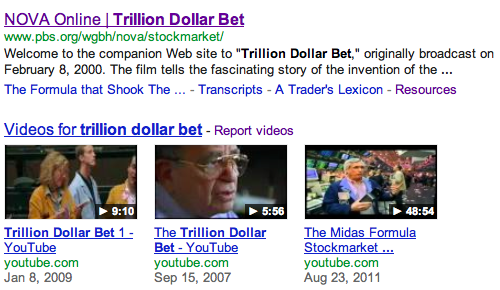
\includegraphics[width=\textwidth]{TrillionDollarBet.png}
        }
        \label{fig:LTCM}
    \end{figure}
\end{frame}

\begin{frame}
    \frametitle{What is Mathematical Modeling?}
    \begin{figure}
        \centering
        \caption{{LAPD Fighting Crime with Math}}
        \href{http://www.youtube.com/watch?v=HZ7fLuO7zb4}{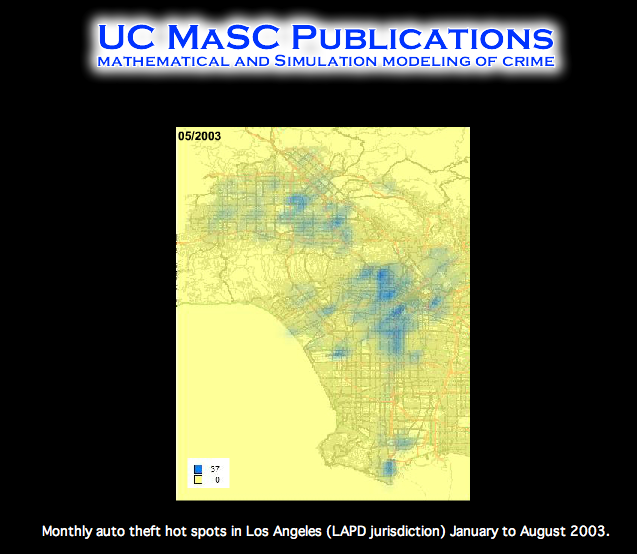
\includegraphics[width=0.6\textwidth]{LAPDUCLA.png}}
        \label{fig:LAPDUCLA}
    \end{figure}
\end{frame}

\begin{frame}[fragile]
    \frametitle{What is Mathematical Modeling?}
        \begin{figure}
            \centering
            \caption{Crime rates and religious beliefs}
            \href{http://www.economist.com/blogs/graphicdetail/2012/09/daily-chart/print}{
            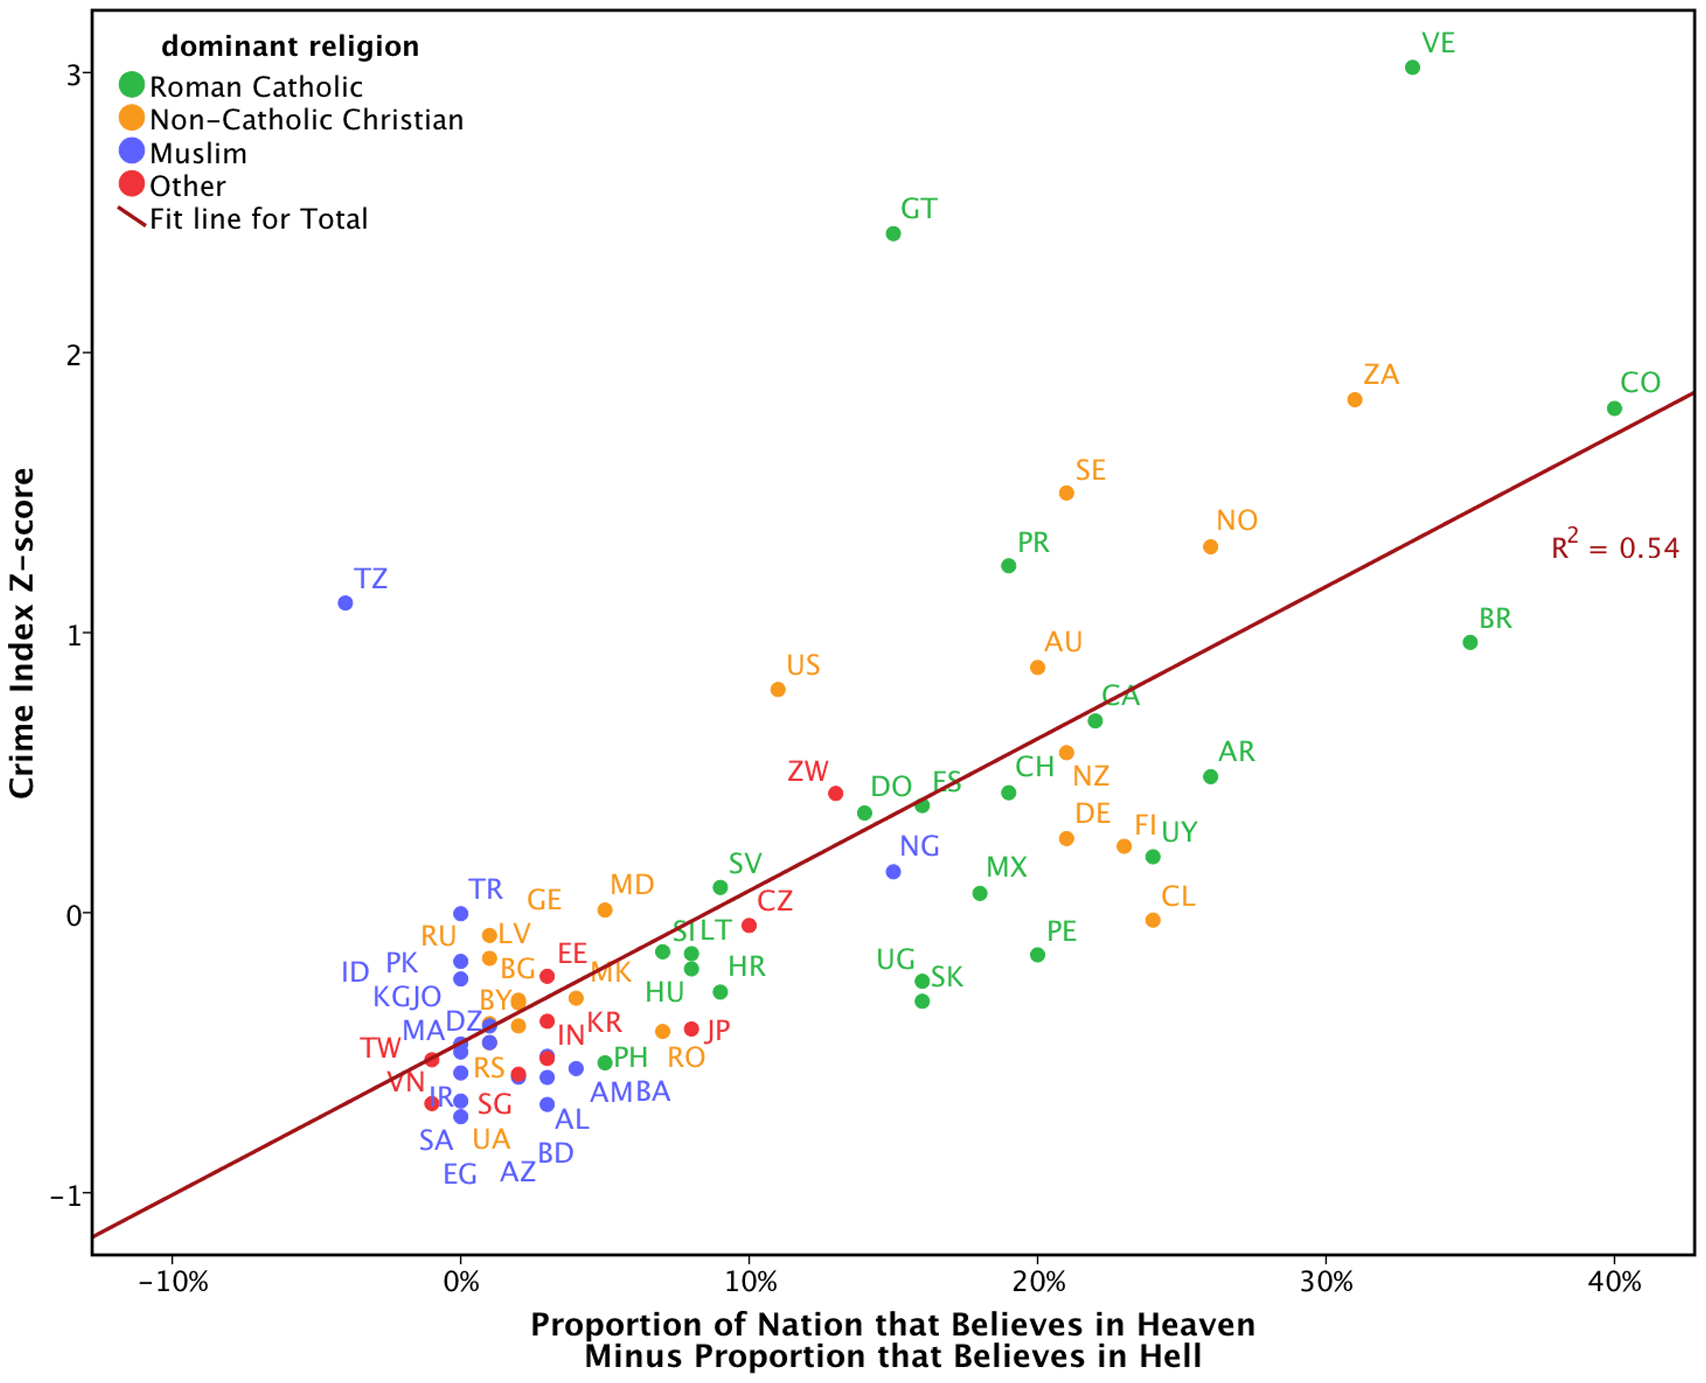
\includegraphics[width=0.7\textwidth]{images/hellvsheaven.png}}
    \end{figure}
\end{frame}

\begin{frame}[fragile]
    \frametitle{More Project Ideas}
    \begin{center}
    \href{http://www.stat.berkeley.edu/users/statlabs/}{http://www.stat.berkeley.edu/}
    \end{center}
    \vskip0.25in
    \begin{center}
        \href{http://www.math.msu.edu/Academic%5FPrograms/graduate/msim//ProjectPage.aspx}{http://www.math.msu.edu/}
    \end{center}
    \vskip0.25in
    \begin{center}
        \href{http://www.mathgoespop.com/2011/09/moneyball.html}{http://www.mathgoespop.com/}
    \end{center}
    \vskip0.25in
    \begin{center}
        \href{http://www.math.hmc.edu/clinic/projects/years/}{http://www.math.hmc.edu/clinic/}
    \end{center}
\end{frame}

\begin{frame}
    \frametitle{Models and Reality}
    \begin{verse}
        The ultimate test of a model is how well it performs when 
        it is applied to the problem it was designed to handle.
    \end{verse}
    \vskip0.5in
    \begin{verse}
       A model is used, it may lead to incorrect predictions. The model is
       often modified, frequently discarded, and sometimes used anyway because
       it is better than nothing. This is the way science develops.  
    \end{verse}
\end{frame}

\begin{frame}
    \frametitle{Models and Reality}
    What makes Mathematical models useful? We must/have/have/have:
    \vskip0.1in
    \begin{itemize}
        \item formulate our ideas precisely and so are less likely to let implicit assumptions slip by,
        \item concise ``language'' which encourages manipulation,
        \item a large number of potential theorems available,
        \item high speed computers available for carrying out calculations.
    \end{itemize}
\end{frame}

\begin{frame}
    \frametitle{Properties of Models}
    As far as a model is concerned, the world can be divided into three parts:
    \vskip0.1in
    \begin{itemize}
        \item Things whose effects are neglected,
        \item Things that affect the model but whose behavior the model is not
            designed to study,
        \item Things the model is designed to study the behavior of. 
    \end{itemize}
\end{frame}
    
\begin{frame}
    \frametitle{A recurring theme}
    Frequently Recurring Elements of doing a Project in Industry:
    \vspace{7pt}
             \begin{enumerate}
                 \item Work Statement,
                 \item Midterm Presentation,
                 \item Progress Report,
                 \item Final Presentation,
                 \item Final Report.
             \end{enumerate}
    \begin{center}
        \href{http://www.ipam.ucla.edu/programs/rips2011/}{
        
\includegraphics[width=0.8\textwidth]{images/ipam}}        
    \end{center}
\end{frame}

\begin{frame}
    \frametitle{What is Work Statement?}
    \begin{itemize}
        \item The written proposal and definition of the project
            \vspace{1cm}
        \item Your consulting team's ``contract'' with the sponsor
            \vspace{1cm}
        \item It is ultimately given to the sponsor for review and signature
    \end{itemize}
\end{frame}



\begin{frame}
    \frametitle{What is Work Statement?}
It sets forth: 
    \begin{itemize}
        \item the nature of the project,
        \item the specific objectives of the project, 
        \item the result expected, 
        \item the ``deliverable'' for the project.
    \end{itemize}
\end{frame}

\begin{frame}
    \frametitle{What is Work Statement?}
    \begin{itemize}
        \item The scope of the project must be within the time table for the
            course
            \vspace{1cm}
        \item The deliverables are reasonable and appropriate
    \end{itemize}
\end{frame}

\begin{frame}
    \frametitle{What is Work Statement?}
    \begin{itemize}
        \item Given the nature of research, it should not include promises
            that your consulting team cannot be certain to achieve
            \vspace{1cm}
        \item It may be necessary after discussion and agreements among
            various parties to modify and renegotiate the work statement as 
            the project progresses
    \end{itemize}
\end{frame}

\begin{frame}
    \frametitle{Example: Insurance Redlining}
    \begin{figure}
        \centering
        \caption{Insurance Redlining}
        \href{http://en.wikipedia.org/wiki/Redlining}{
        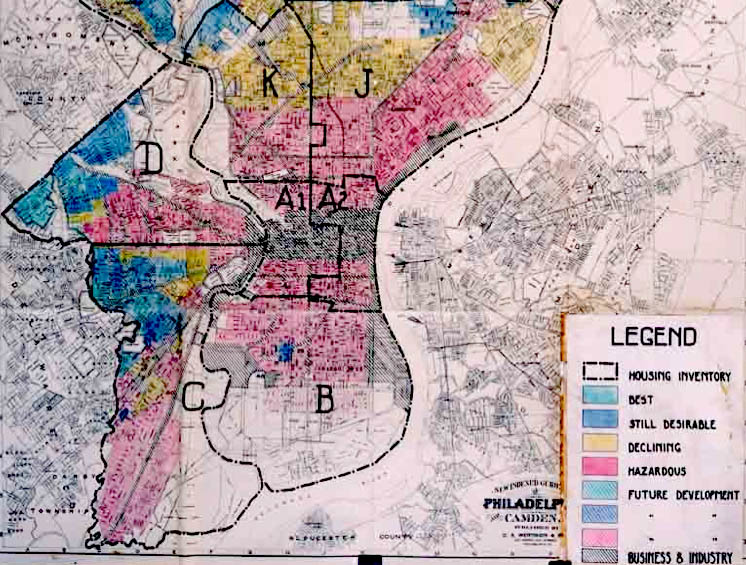
\includegraphics[width=0.8\textwidth]{redliningPhilly.jpg}
        }
                \label{fig:redlining}
    \end{figure}
\end{frame}




\newtheorem{DEFinsredlining}{Insurance Redlining}
\newtheorem{DEFfairplan}{FAIR}
\begin{frame}
    \frametitle{Example: Insurance Redlining}
    \begin{DEFinsredlining}
        \textcolor{red}{Insurance redlining} refers to the practice of refusing
        to issue insurance to certain types of people or within some 
        geographic area. 
    \end{DEFinsredlining}
\vskip.5in
    \begin{DEFfairplan}
        The \textcolor{red}{FAIR} plan was offered by the city of Chicago as a 
        default policy to homeowner who had been rejected by the voluntary
        market. 
    \end{DEFfairplan}
\end{frame}

\newtheorem{DEFsponsorUSCCR}{Sponsor}
\newtheorem{DEFdataFAIR}{Data}
\begin{frame}
    \frametitle{Example: Insurance Redlining}
    \begin{DEFsponsorUSCCR} 
        The \href{http://www.usccr.gov/about/}{\textcolor{red}{U.S.~Commission
        on Civil Rights}} examined 
        charges by several Chicago community organizations that insurance 
        companies were redlining their neighborhoods. 
    \end{DEFsponsorUSCCR}
    \vskip.5in
    \begin{DEFdataFAIR}
        The \textcolor{red}{number of FAIR plan policies} written and renewed in Chicago
        by zip code for the number of months of December 1977 through May
        1978.
    \end{DEFdataFAIR}
\end{frame}

\begin{frame}
    \frametitle{Example: Insurance Redlining}
    Variables to consider:
    \begin{description}
        \item[\texttt{race}] Racial composition in percentage of minority,
        \item[\texttt{fire}] Fire per 100 housing units,
        \item[\texttt{theft}] Theft per 100 housing units,
        \item[\texttt{age}] Theft per 1000 population,
        \item[\texttt{involact}] New FAIR plan policies and renewal per 100 housing units,
        \item[\texttt{income}] Median family income in thousands of dollars,
        \item[\texttt{side}] North or South side of Chicago.
    \end{description}
\end{frame}

\begin{frame}
    \frametitle{Work Statement: Introduction}
    Describe:
    \begin{itemize}
        \item the purpose of the project,
        \item a brief introduction of the sponsoring organization,
        \item a suitably condensed statement of the problem,
        \item some discussion of the relevance of the project to the sponsor.
    \end{itemize}
\end{frame}

\begin{frame}[fragile]
    \frametitle{Work Statement: Introduction}
    The work statement should contain a short description 
    of your sponsor.  
    \vskip0.2in
    For the insurance redlining example, 
    \emph{U.S.~Commision on Civil Rights} would be the sponsor.
    \vskip0.2in
    \href{http://en.wikipedia.org/wiki/Boilerplate_%28text%29}{\emph{Boilerplating}} from the sponsor's webpage is often acceptable. 
    \vskip0.5in
    \begin{center}
        \href{http://www.usccr.gov/about/}{http://www.usccr.gov}
    \end{center}
\end{frame}

\begin{frame}   
    \frametitle{Work Statement: Problem Statement}
    \begin{verse}
        Can the insurance companies claim that the discrepancy is due to 
        greater risks in some zip codes?
    \end{verse}
    \vskip0.5in
    \begin{verse}
        The insurance companies could claim that they were denying insurance 
        in neighborhoods where they had sustained large fire-related losses
        and any discriminatory effect was a by-product of legitimate business
        practice.  
    \end{verse}
\end{frame}

\begin{frame}[fragile]
    \frametitle{Work Statement: Timeline \& Deliverable}
    \begin{verse}
        ``When I decide the time needed for the project,
        I first approximate the time that I might actually need, 
        and then, request the sponsor the double of the approximated time.''
    \end{verse}
    \vskip0.3in
    \begin{description}
        \item[From Team to Sponsor] Presentations, Reports, Special Softwares.
            \vskip0.5in
        \item[From Sponsor to Team] Regular meetings, Data \& Contingences,
            Code \& Code Documentation.
    \end{description}
\end{frame}

\newtheorem{DEFecofallacy}{Ecological Fallacy}
\begin{frame}
    \frametitle{Example: Ecological Fallacy}
    \begin{DEFecofallacy}
       When data are collected at the group level, we may observe 
       a correlation between two variables.  The \textcolor{red}{ecological
       fallacy} is concluding that the same correlation holds at the
       individual level. 
    \end{DEFecofallacy}
\end{frame}

\begin{frame}
    \frametitle{Example: Ecological Fallacy}
    \begin{figure}
        \centering
        \caption{1998 annual per capita income and proportion U.S.~born for 50
        states plus D.C.}
        \includegraphics[width=0.75\textwidth]{images/FigureFarawayFigure11dot1.png}
    \end{figure}
\end{frame}

\begin{frame}
    \frametitle{Example: Ecological Fallacy}
    \begin{figure}
        \centering
        \caption{1998 annual per capita income and proportion U.S.~born for 50
        states plus D.C.}
        \includegraphics[width=0.75\textwidth]{images/FigureFarawayFigure11dot1b.png}
    \end{figure}
\end{frame}

\begin{frame}[fragile]
    \frametitle{Example: Insurance Redlining}
    \begin{verse}
For the ecological fallacy example, 
the assumption would be that the incomes of 
the native born do not depend on the proportion of native 
born within the state (and similarly for naturalized citizens).
    \end{verse}
    \vskip0.5in
    \begin{verse}
        For the insurance redlining example, we only have aggregate data.  
        We must inform the sponsor that unless more detailed data becomes
        available, the results for the aggregated data may not hold true 
        at the individual level. 
    \end{verse}
\end{frame}

\begin{frame}
    \frametitle{Presentations in this class}
    \begin{figure}
        \caption{For your presentation recording needs}
        \href{https://know.it.jhu.edu/display/TECHCLASS/Homewood+Campus}{
        
\includegraphics[width=0.7\textwidth]{images/BLC2006.jpg}}
    \end{figure}
\end{frame}
            
\begin{frame}
    \frametitle{Programmings in this class}
    \begin{itemize}
        \item \LaTeXs: 
            \begin{itemize}
                \item \texttt{moderncv}
                \item \texttt{beamer}
                \item \texttt{report}
                \item \href{http://www.texample.net}{\texttt{pgf/TikZ}}
            \end{itemize}
        \item Git
            \begin{itemize}
                \item \href{http://git-scm.com/doc}{\texttt{git gui}}
            \end{itemize}
        \item R:
            \begin{itemize}
                \item \texttt{lm}
                \item \href{https://catalyst.library.jhu.edu/catalog/bib_3642743}{\texttt{ggplot2}}
                \item \href{http://www.texample.net/tikz/examples/tikzdevice-demo/}{\texttt{tikzDevice}}
                \item \href{http://www.public.iastate.edu/~dicook/VIGRE/R-packages-slides.pdf}{\texttt{R CMD build}}
            \end{itemize}
    \end{itemize}
\end{frame}


\begin{frame}[fragile]
    \frametitle{Where to get some help for \LaTeXs}
    \begin{center}
    \href{http://en.wikibooks.org/wiki/LaTeX/}{http://en.wikibooks.org/wiki/LaTeX/}
    \end{center}
\end{frame}

\begin{frame}[fragile]
    \frametitle{Tutorial: \LaTeXs}
    \LaTeXs is a computer language for writing a scholarly paper:
    \begin{table}
        \centering
        \caption{HTML vs \LaTeXs}
        \begin{tabular}{c|p{3cm}|p{3cm}}
            \quad   &   HTML    & \LaTeXs \\ 
            \hline
            Code    & 
            \begin{lstlisting}
<html> 
 . . .
</html>
            \end{lstlisting} &  
            \begin{lstlisting}
\begin{document}
 . . .
\end{document}
            \end{lstlisting}\\
            \hline
            Compiler & Firefox and etc. & pdflatex and etc. \\
            \hline
            Output  & Web-page & PDF file
        \end{tabular}
        \label{tab:htmlvslatex}
    \end{table}
\end{frame}

\begin{frame}
    \frametitle{Tutorial: \LaTeXs}
    TeXworks is:
    \begin{itemize}
        \item an editing tool that is separate from \LaTeX,
        \item available in Linux, OSX and Windows,
        \item avaiable in: 
    \end{itemize}
    \vskip0.3in
    \begin{center}
    \href{http://code.google.com/p/texworks/}
    {http://code.google.com/p/texworks/}
    \end{center}
\end{frame}


\begin{frame}[fragile]
    \frametitle{Tutorial: \LaTeXs}
    \begin{itemize}
        \item Demo on preparing a resume using \LaTeXs \texttt{moderncv} package:
            \begin{itemize}
                \item Install \LaTeXs (MikTeX in Windows and MacTeX in OSX),
                \item Download \texttt{moderncv} package files from the course folder,
                \item Change file names to reflect you,
                \item Edit the TeX file,
                \item Compile using your favorite \LaTeXs editor,
                \item Look at the resulting PDF file.
            \end{itemize}
    \end{itemize}
\end{frame}

\begin{frame}[fragile]
    \frametitle{Cautions: \LaTeXs}
    There are numerous quirky \LaTeXs rules:
    \begin{itemize}
        \item opening quotation is not the same as the closing quotation,
        \item period yields \emph{two} blank spaces, 
        \item for \%, need to type \verb+\%+,
        \item for \textbackslash, need to type \verb+\textbackslash+,
        \item for /, need to type /,
        \item for \{, need to type \verb+\{+,
        \item for \$, need to type \verb+\$+,
        \item \verb+~+ yields a single blank space,
        \item and etc.
    \end{itemize}
\end{frame}

\newtheorem{POEMbender}{The Blind Men and the Elephant}
\begin{frame}[fragile]
    \frametitle{Demo: \LaTeXs + Git}
    \begin{POEMbender}
       \quad 
    \end{POEMbender}
        \begin{itemize}
            \item Start up a git folder
            \item Create and edit the \texttt{.gitignore} file
            \item Download the template for a beamer file
            \item Look up the poem from the book
            \item One slide per stanza
            \item Compile after each stanza
            \item Commit after creating each stanza
            \item Repeat until done.
        \end{itemize}
\end{frame}

\begin{frame}[fragile]
    \frametitle{Tutorial: Git}

\begin{lstlisting}
sudo apt-get install git
\end{lstlisting}

\begin{figure}[b]
    \caption{An alternative: \texttt{git gui}}
    \begin{center}
        
\includegraphics[height=0.6\textheight]{gitguiinstall.png}
    \end{center}
    \label{fig:gitgui}
\end{figure}
    
\end{frame}

\begin{frame}[fragile]
    \frametitle{Tutorial: Git}

\vspace{8pt}
\begin{lstlisting}
cd ~/
git clone http://cis.jhu.edu/~nhlee/550400.git
\end{lstlisting}

\begin{figure}[b]
    \caption{An alternative: \texttt{git gui}}
    \begin{center}
        
\includegraphics[height=0.5\textheight]{gitgui.png}
    \end{center}
    \label{fig:gitgui2}
\end{figure}
    
\end{frame}

\begin{frame}[fragile]
    \frametitle{Tutorial: Git}
\begin{lstlisting}
cd ~/550400.git
git reset --hard HEAD
git pull origin master
\end{lstlisting}
\begin{figure}[b]
    \centering
    \caption{An alternative: \texttt{git gui}}
        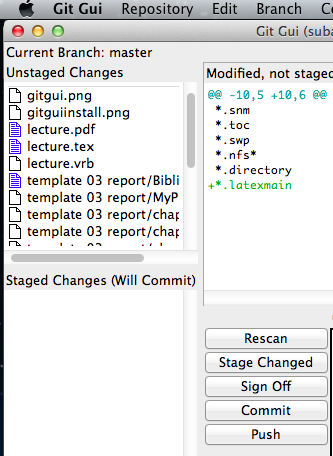
\includegraphics[height=0.6\textheight]{gitguiusing.png}
    \label{fig:gitgui4}
\end{figure}
    
\end{frame}

\begin{frame}
    \frametitle{Tutorial: Git}
    \begin{itemize}
        \item Demo I: build a \emph{personal} Git folder 
            \begin{itemize}
                \item Create some files
                \item Stage the files 
                \item Commit the files
            \end{itemize}
        \item Demo II: build the \emph{course} Git folder
    \end{itemize}
\end{frame}

\begin{frame}[fragile]
    \frametitle{Unofficial Way to Access the Course Folder}
    \vskip0.5in
    \begin{center}
        \href{http://cis.jhu.edu/~nhlee/550400.html/}{
            \url{http://cis.jhu.edu/~nhlee/550400.html/}
        }
    \end{center}
\end{frame}

\begin{frame}[fragile]
    \frametitle{Demo: R}
    \begin{columns}
        \begin{column}{0.5\textwidth}
            \begin{figure}
                \centering
            \caption{R Studio}
            \href{http://rstudio.org}{
            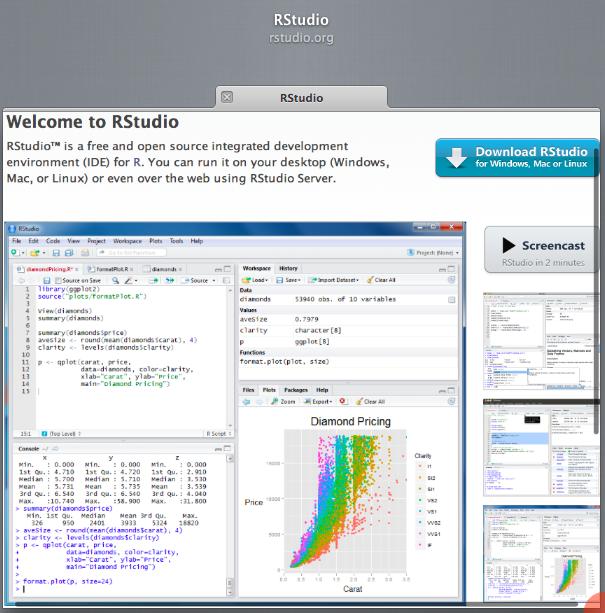
\includegraphics[width=\textwidth]{images/Rstudio}
            }
        \end{figure}
        \end{column}
        \begin{column}{0.5\textwidth}
            \begin{figure}
                \centering
                        \caption{R}
                    \href{http://www.r-project.org}{
                        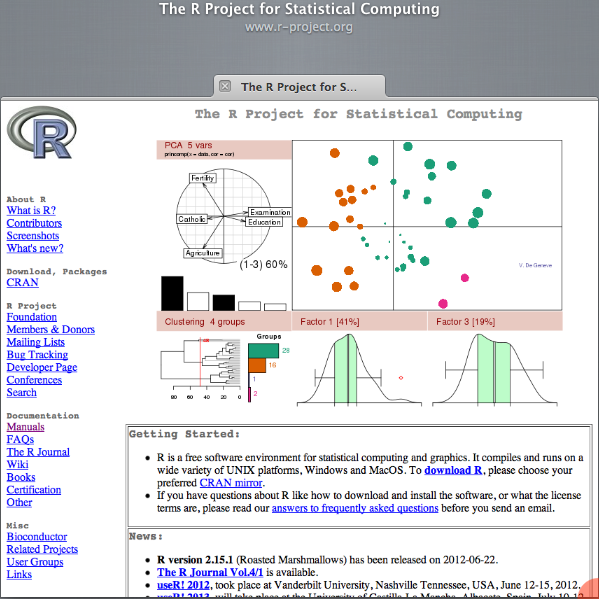
\includegraphics[width=\textwidth]{images/Rproject}}
            \end{figure}
        \end{column}
    \end{columns} 
\end{frame}

\begin{frame}[fragile]
    \frametitle{Demo: R}
    \begin{columns}
        \begin{column}{0.5\textwidth}
    \begin{lstlisting}
install.packages(faraway)
require(faraway)
data(eco)
plot(income ~ usborn, 
    data=eco,
    xlab=`Proportion US born'
    ylab=`Mean Annual Income'
    )
    \end{lstlisting}
        \end{column}
        \begin{column}{0.5\textwidth}
            \includegraphics[width=\textwidth]{FigureFarawayFigure11dot1.png}
        \end{column}
    \end{columns} 
\end{frame}

\begin{frame}[fragile]
    \frametitle{Demo: R}
    \begin{columns}
        \begin{column}{0.5\textwidth}
            \begin{lstlisting}
g <- lm(income ~ usborn, eco) 
summary(g)
plot(income ~ usborn, 
    data = eco,
    xlab=`Proportion US born',
    ylab=`Mean Annual Income',
    xlim=c(0,1),
    ylim=c(15000,70000),
    xaxs='i')
abline(coef(g))
            \end{lstlisting}
        \end{column}
        \begin{column}{0.5\textwidth}
            \includegraphics[width=\textwidth]{FigureFarawayFigure11dot1b.png} 
        \end{column}
    \end{columns} 
\end{frame}

\begin{frame}[fragile]
    \frametitle{Example: Insurance Redlining}
\begin{lstlisting}
data(chredlin);
chredlin;
head(chredlin);
summary(chredlin);
par(mfrow=c(1,1));
pairs(chredlin);
summary(lm(involact ~ race, chredlin));
plot(involact ~ race, chredlin);
abline(lm(involact ~ race, chredlin));
plot(fire ~ race, chredlin);
abline(lm(fire ~ race, chredlin));
\end{lstlisting}
\end{frame}


\section{Principles}
\begin{frame}
    \frametitle{Seven Basic Principles}
     \begin{enumerate}
         \item Set the context 
         \item Choose effective examples and analogies
         \item Choose vocabulary to suit your readers
         \item Decide whether to present \#s in text, tables, or figures
         \item Report and interpret \#s in the text
         \item Specify the direction \emph{and} size of an association between variables
         \item For many \#s, summarize overall pattern 
     \end{enumerate}
\end{frame}

\section{Tools}
\begin{frame}
    \frametitle{Creating Effective Tables}
    
\end{frame}

\section{Arguments from Scale}

\begin{frame}
    \frametitle{Example: Cost of Packaging}
\end{frame}

\section{Graphical Methods}
\begin{frame}
    \frametitle{Example: The Nuclear Mission Arms Race}
    
\end{frame}

\section{Basic Optimization}
\begin{frame}
    \frametitle{Example: Maintaining Inventory}
    
\end{frame}
\end{document}
